\documentclass{beamer}
\usepackage{amsmath, amssymb, bm}
\usepackage{graphicx}
\usepackage{hyperref}

\usetheme{Berlin}

\title{Polya-Gamma Distribution and Data Augmentation}
\author{Toni Luhdo}
\date{\today}

\begin{document}
	
	\frame{\titlepage}
	
	\begin{frame}{Introduction}
		\begin{itemize}
			\item Logistic regression is a fundamental model for classification problems.
			\item Bayesian inference requires efficient sampling methods.
			\item The Polya-Gamma distribution enables an elegant solution to the Gibbs sampling strategy.
		\end{itemize}
	\end{frame}
	
	
	\begin{frame}{Polya-Gamma Distribution}
			\textbf{Definition:} A random variable $\omega$ is called Polya-Gamma distributed with parameters \( b \) and \( c \) if it has the following density function:
			\begin{equation}
			f(x \mid b, c) = \{\cosh^b(c/2)\} \frac{2^{b-1}}{\Gamma(b)}
			\sum_{n=0}^{\infty} (-1)^n 
			\frac{\Gamma(n + b) (2n + b)}{\Gamma(n + 1) \sqrt{2\pi} x^3} 
			e^{- \frac{(2n+b)^2}{8x} - \frac{c^2}{2}x}
		\end{equation}
		for $x > 0$.\\
		\textbf{Remark}
		If c = 0 we get the so called standard Polya-Gamma density:
			\begin{equation}
			f(x \mid b, 0) = \frac{2^{b-1}}{\Gamma(b)}
			\sum_{n=0}^{\infty} (-1)^n 
			\frac{\Gamma(n + b) (2n + b)}{\Gamma(n + 1) \sqrt{2\pi} x^3} 
			e^{- \frac{(2n+b)^2}{8x}}
		\end{equation}
	\end{frame}
	
	\begin{frame}{Polya-Gamma Distribution}
		
%		\textbf{Definition:} A random variable $\omega$ is called Polya-Gamma distributed with parameters \( b \) and \( c \) if it has the following density function:
%		\begin{equation}
%			p(\omega | b, c) = \frac{\exp(-c^2 \omega /2) p(\omega | b, 0)}{E_{PG(b,0)}[\exp(-c^2 \omega /2)]}
%		\end{equation}
%		where $p(\omega | b, 0)$ is the standard Polya-Gamma density.
		%		Defined by... and Gamma function
		%		Standard Polya-Gamma specification
		\begin{itemize}
			\item \( b \in \mathbb{R}^{+}, \quad b > 0 \) Controls the shape of the distribution (shape parameter).
			\item \( c \in \mathbb{R}\) Influences the scaling/tilt (scale parameter).
			\item \( \Gamma(x) = \int_0^\infty t^{x-1} e^{-t} dt, \quad \text{for } x > 0 \)
		\end{itemize}
	\end{frame}
	
	\begin{frame}
		\begin{figure}
			\centering
			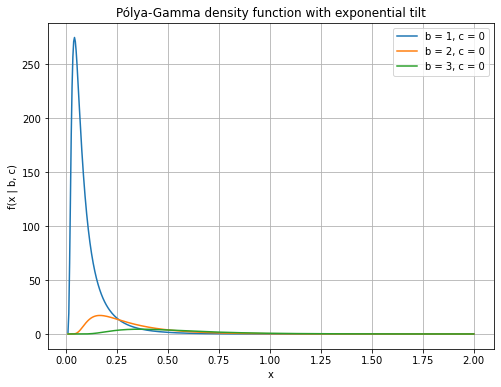
\includegraphics[width=0.95\linewidth]{polya_b1c0}
			\label{fig:polyab1c0}
		\end{figure}
	\end{frame}
	
	
	\begin{frame}{Laplace Transformation Properties}
		A different representation of the polya gamma distribution is given by
				\begin{equation}
			p(\omega | b, c) = \frac{\exp(-c^2 \omega /2) p(\omega | b, 0)}{E_{PG(b,0)}[\exp(-c^2 \omega /2)]}
		\end{equation}
		The Laplace transform of the Polya-Gamma distribution is given by:
		\begin{equation}
			E[\exp(-\omega t)] =\frac{ \cosh^{b}(c/2)}{\cosh^{b}(\sqrt{\frac{c^2/2+t}{2}})}
		\end{equation}
		\begin{itemize}
			\item Useful for analytical computations and simulations.
			\item Basis for MCMC methodology in Bayesian inference.
		\end{itemize}
	\end{frame}
	




	\begin{frame}{Alternative Representation of the Polya-Gamma Distribution}
		\begin{itemize}
			\item The distribution can be represented as an infinite sum of gamma-distributed variables:
			\begin{equation}
				\omega \sim \sum_{k=1}^{\infty} \frac{G_k}{(k - 1/2)^2 + c^2/(4  \pi^2)}, \quad G_k \sim \text{Gamma}(b,1)
			\end{equation}
			\item This representation highlights the relationship to the gamma distribution and offers alternative computational approaches.
		\end{itemize}
	\end{frame}
	
	\begin{frame}{Properties of the Polya-Gamma Class}
		\begin{itemize}
			\item Closed under convolution: If $\omega_1 \sim PG(b_1, z)$ and $\omega_2 \sim PG(b_2, z)$ are independent, then:
			\begin{equation}
				\omega_1 + \omega_2 \sim PG(b_1 + b_2, z)
			\end{equation}
			\item Expectation:
			\begin{equation}
				E(\omega) = \frac{b}{2c} \tanh(c/2)
				%				, \quad \text{Var}(\omega) = \frac{b}{4c^3} \text{sech}^2(c/2)
			\end{equation}
		\end{itemize}
	\end{frame}
	
	\begin{frame}{Bayesian Inference for Logistic Models}
		The likelihood function of a logistic model is:
		\begin{equation}
			P(y_i = 1 | x_i, \beta) = \frac{1}{1 + e^{-x_i^T \beta}}
		\end{equation}
		\begin{itemize}
			\item Introducing a latent Polya-Gamma parameter $\omega_i$ enables a Gibbs sampling method.
			\item The posterior distribution is normal for $\beta$ and Polya-Gamma for $\omega$.
		\end{itemize}
	\end{frame}
	
	\begin{frame}{Transformation of the Likelihood with Polya-Gamma}
		The likelihood function of a logistic model is originally given by:
		\begin{equation}
			P(y_i = 1 | x_i, \beta) = \frac{1}{1 + e^{-x_i^T \beta}}
		\end{equation}
		Using Polya-Gamma data augmentation, we utilize the identity:
		\begin{equation}
			\frac{e^{y_i x_i^T \beta}}{1 + e^{x_i^T \beta}} = \int_0^\infty e^{-\omega_i (x_i^T \beta)^2 / 2} p(\omega_i | 1, 0) d\omega_i
		\end{equation}
		This allows the likelihood to be rewritten in a form that results in a conditional normal distribution for $\beta$, enabling Gibbs sampling.
	\end{frame}
	
	\begin{frame}{Gibbs Sampler for the Logistic Model}
		\begin{enumerate}
			\item Sample $\omega_i | \beta \sim PG(n_i, x_i^T \beta)$ for all $i$.
			\item Sample $\beta | z, \omega \sim N(m_{\omega}, V_{\omega})$, where:
			\begin{equation}
				m_{\omega} = V_{\omega} X^T \kappa, \quad V_{\omega} = (X^T \Omega X + B^{-1})^{-1}
			\end{equation}
		\end{enumerate}
		with $\kappa = (y_1 - n_1/2, ..., y_N - n_N/2)$, and $\Omega$ being the diagonal matrix of $\omega_i$. \\ 
		$B$ is the prior covariance matrix for the coefficients $\beta$.
	\end{frame}
	
	\begin{frame}{The Gutenberg-Richter Law for Earthquakes}
		\begin{itemize}
			\item An empirical law describing the relationship between earthquake magnitude and frequency.
			\item Proposed by Charles Francis Richter and Beno Gutenberg (1956).
			\item Gutenberg-Richter Law:
			\begin{center}
				\textcolor{red}{$ \log_{10}(N) = a - bM $}
			\end{center}
			\item $N$ is the cumulative annual number of earthquakes with a magnitude greater than $M$.
			\item $a$ represents the total seismicity rate of the observed region.
			\item $b$ expresses the relative proportion of small to large earthquakes.
		\end{itemize}
	\end{frame}
	
	
	\begin{frame}
		\begin{figure}
			\centering
			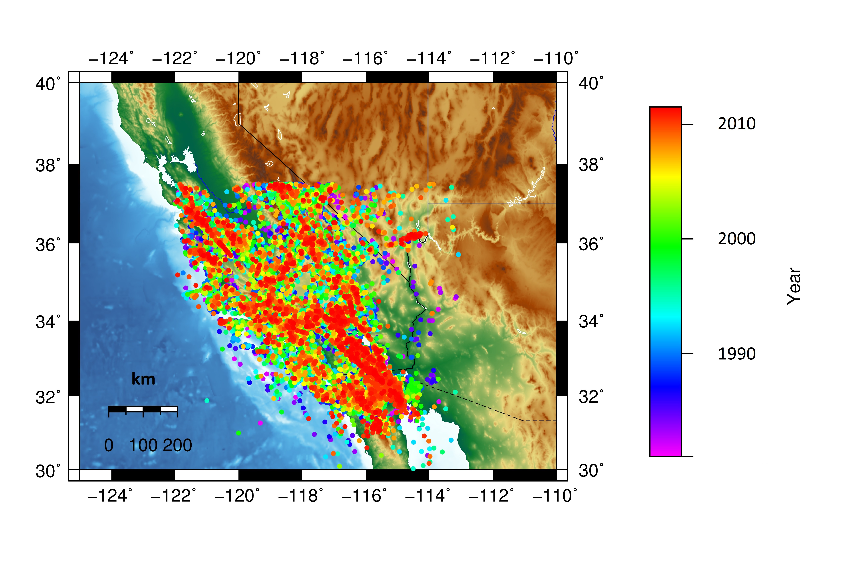
\includegraphics[width=0.95\linewidth]{erdbeben1}
			\label{fig:earthquake1}
		\end{figure}
	\end{frame}
	
	\begin{frame}
		\begin{figure}
			\centering
			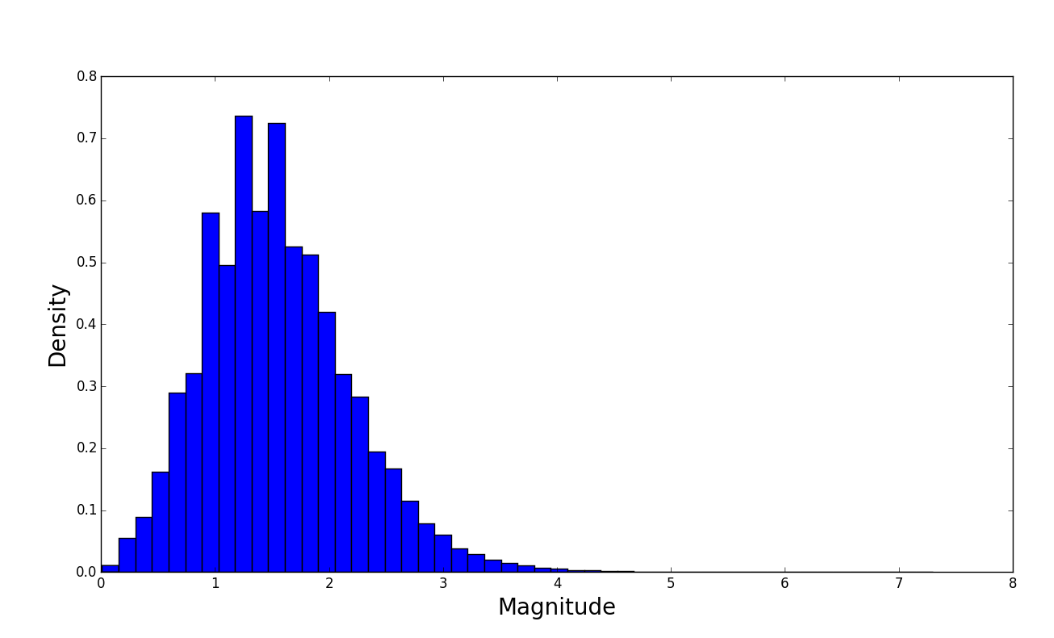
\includegraphics[width=0.95\linewidth]{erdbeben2}
			\label{fig:earthquake2}
		\end{figure}
	\end{frame}
	
	\begin{frame}
		\begin{figure}
			\centering
			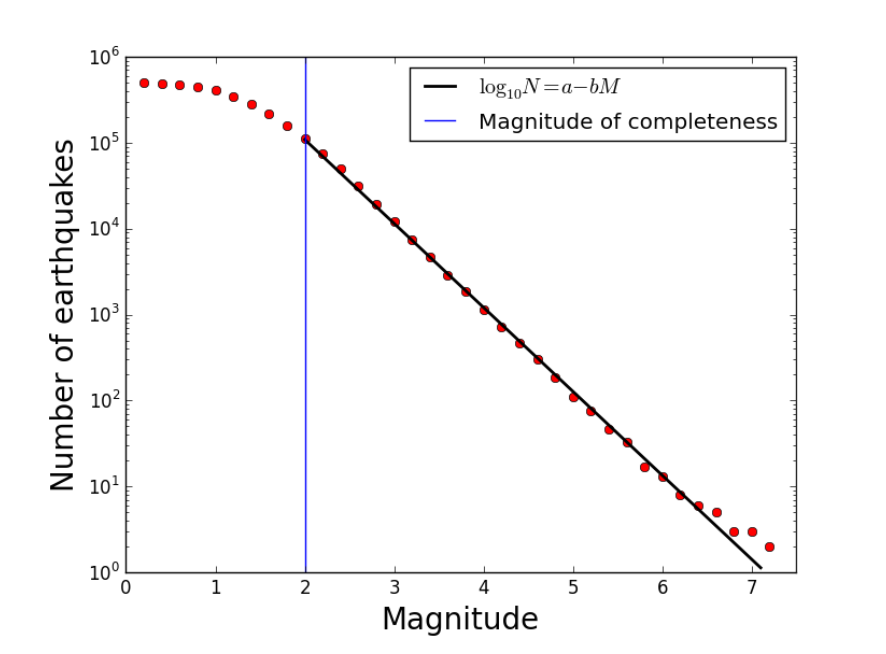
\includegraphics[width=0.95\linewidth]{erdbeben3}
			\label{fig:earthquake3}
		\end{figure}
	\end{frame}
	
%	\begin{frame}{Estimating $b$ with Polya-Gamma Data Augmentation}
%		\begin{itemize}
%			\item The Bayesian estimation of $b$ can be performed using Polya-Gamma data augmentation.
%			\item By transforming the likelihood function into a logistic model:
%			\begin{equation}
%				P(y_i = 1 | m_i, b) = \frac{1}{1 + e^{-m_i b}}
%			\end{equation}
%			the Polya-Gamma method can be utilized for efficient Gibbs sampling.
%			\item This approach may help obtain robust estimates for seismic activity parameters.
%		\end{itemize}
%	\end{frame}
	
	
	\begin{frame}{Estimating $b$ with Polya-Gamma Data Augmentation}
		\begin{itemize}
			\item The Bayesian estimation of the parameter $b$ can be facilitated using Polya-Gamma data augmentation.
			\item By transforming the Gutenberg-Richter equation into a logistic model:
			\begin{equation}
				P(y_i = 1 | m_i, b) = \frac{1}{1 + e^{-m_i b}}
			\end{equation}
			the Polya-Gamma method can be used to develop a Gibbs sampling strategy for determining $b$.
			\item Advantages of this method:
			\begin{itemize}
				\item It enables a robust estimation of $b$, even with small or noisy data.
				\item The Bayesian approach allows for direct quantification of uncertainties in the estimation.
				\item It provides a natural way to incorporate additional prior information about $b$.
			\end{itemize}
		\end{itemize}
	\end{frame}
	
	\begin{frame}{Why Use Polya-Gamma for Estimation?}
		\begin{itemize}
			\item Modeling earthquake frequency as a Poisson process:
			\[ N(M) \sim \text{Poisson}(\lambda(M)) \]
			
			\item Log transformation leads to a linear model:
			\[ \log N(M) = a - bM \]
			\item The Polya-Gamma method enables Gibbs sampling for estimation.
		\end{itemize}
	\end{frame}
	
	\begin{frame}{Summary}
		\begin{itemize}
			\item The Polya-Gamma distribution significantly simplifies Bayesian inference for logistic models.
			\item The Gibbs sampling strategy allows for efficient numerical computations.
			\item The method is well-suited for large-scale data analysis and machine learning.
		\end{itemize}
	\end{frame}
	
	
	\begin{frame}{References}
		Polson, N. G., Scott, J. G., Windle, J. (2013). Bayesian inference for logistic models using Polya-Gamma latent variables. \textit{Journal of the American Statistical Association}, 108(504), 1339-1349.
	\end{frame}
	
	\begin{frame}
		Thanks for your Attention!
	\end{frame}
	
	
	\begin{frame}{Appendix: Meaning of the Parameters $b$ and $c$ in the Polya-Gamma Distribution}
		\begin{itemize}
			\item **Parameter $b$ (Shape Parameter):**
			\begin{itemize}
				\item Determines the scaling of the distribution.
				\item Higher values make the distribution narrower and more concentrated.
				\item Often derived from the number of trials in the model.
			\end{itemize}
			\item **Parameter $c$ (Scale Parameter):**
			\begin{itemize}
				\item Controls the exponential damping.
				\item Higher values of $c$ shift the distribution to the left.
				\item In logistic models, $c = x^T \beta$.
			\end{itemize}
		\end{itemize}
	\end{frame}
	
	\begin{frame}{Appendix: Effects of $b$ and $c$ on the Distribution}
		\begin{itemize}
			\item If $b = 1$ and $c = 0$: The distribution resembles a Gamma distribution.
			\item If $c$ increases: The distribution shifts to the left.
			\item If $b$ increases: The distribution becomes narrower and more concentrated.
		\end{itemize}
		\centering
		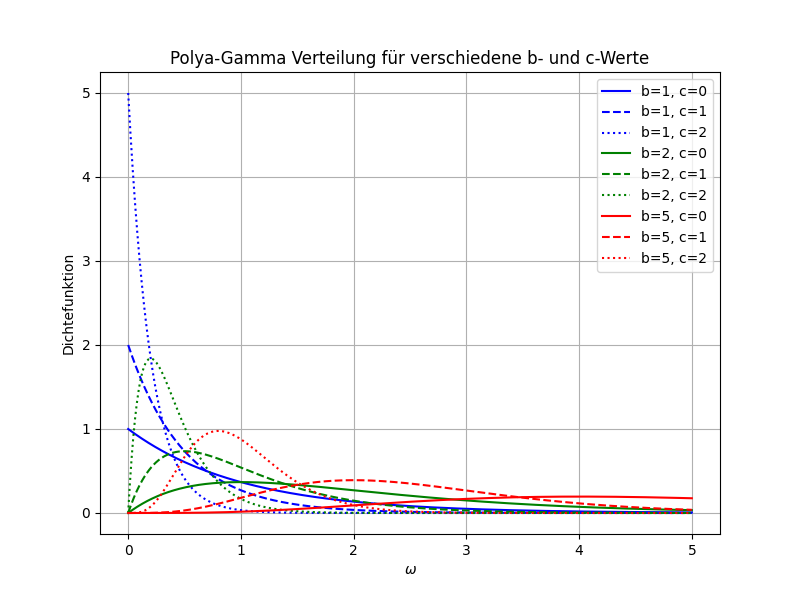
\includegraphics[width=0.6\textwidth]{polya_gamma_distribution.png}
	\end{frame}
	
	\begin{frame}{Appendix: Why is $p(\omega_i | 1, 0)$ in the Likelihood Transformation?}
		\begin{itemize}
			\item In logistic regression, the likelihood is given by:
			\begin{equation}
				P(y_i = 1 | x_i, \beta) = \frac{1}{1 + e^{-x_i^T \beta}}
			\end{equation}
			\item Using the Polya-Gamma transformation, this is rewritten as:
			\begin{equation}
				P(y_i = 1 | x_i, \beta) = \int_0^\infty e^{-\omega_i (x_i^T \beta)^2 / 2} p(\omega_i | 1, 0) d\omega_i
			\end{equation}
			\item **Why $PG(1,0)$?**
			\begin{itemize}
				\item $b = 1$ because it is a binary logistic regression (Bernoulli model).
				\item $c = 0$ because no exponential damping is required.
			\end{itemize}
		\end{itemize}
	\end{frame}
\end{document}